\documentclass[preprint,12pt,times,numafflabel]{elsarticle}
\usepackage[T1]{fontenc}
\usepackage{booktabs,tabularx,array,amsmath,amssymb,graphicx,placeins,url,float,siunitx,multirow}
\usepackage[hidelinks]{hyperref}
\graphicspath{{../figures/}}
\newcommand{\RefA}{\textsc{Reference}}
\newcommand{\Cor}{\textsc{Corrected}}
\newcommand{\Guard}{\textsc{Guard}}
\emergencystretch=6em
\journal{Preprint (revised after internal evidence audit; not yet submission-ready)}

\begin{document}
\begin{frontmatter}
\title{Routing-Aware Federated Learning for IoT Intrusion Detection under Client Failures and Sign-Flip Attackers: A Reproducible Simulation Study of Delivery Reliability, Participation Fairness and Stability}

\author[1]{Nahideh Derakhshanfard}
\author[1]{Reza Azarnia}
\author[2]{Amir Mollanejad}
\author[3]{Ali Asghar Pour Haji Kazem}
\author[4]{Neda Dadashkhani}
\author[5]{Parisa Khoshvaght}
\author[6]{Mehdi Hosseinzadeh}
\address[1]{Department of Computer Engineering, Tabriz Branch, Islamic Azad University, Tabriz, Iran}
\address[2]{Department of Computer Engineering, Aras Branch, Islamic Azad University, Jolfa, Iran}
\address[3]{Department of Software Engineering, Faculty of Engineering and Natural Sciences, Istinye University, Istanbul, Turkey}
\address[4]{Computer Programming Program, Vocational School, Istinye University, Istanbul, Turkey}
\address[5]{Institute of Research and Development, Duy Tan University, Da Nang, Vietnam}
\address[6]{School of Engineering \& Technology, Duy Tan University, Da Nang, Vietnam}

\begin{abstract}
Federated intrusion detection over edge--cloud IoT networks must cope with unreliable delivery, failed clients and poisoned updates, and design choices that help one of these concerns often hurt another. We report a controlled simulation study of a routing-aware federated pipeline (route-scored client selection, a packet-level delivery model, median/MAD update filtering, surrogate imputation of missing updates, server momentum and an optional Gaussian perturbation) on UNSW-NB15 and CICIoT2023. The protocol is validation-only, three-way and group-disjoint (final-test data were not used); 24 arms were run with five paired seeds each (240 runs), plus a 40-run follow-up on UNSW-NB15 (seeds 17--21). Our findings are: (i) 20\% sign-flip clients make undefended FedAvg collapse (UNSW-NB15 last-round ROC-AUC $0.60$--$0.65$), whereas the MAD filter with server momentum recovers $0.984$ (best checkpoint), indistinguishable from clean FedAvg ($0.984$); (ii) deterministic top-k routing raises the mean packet delivery ratio from $0.782$ (uniform selection) to $0.851$ and shortens delay by 6.0\% (UNSW-NB15 trace), but leaves 27.2 of 50 clients unselected (selection Gini $0.731$ vs.\ $0.205$); coverage-aware selection restores part of the participation (Gini $0.486$, 8.0 unselected clients) at PDR $0.833$ without a measurable AUC change; (iii) a bundle of changes intended to correct the reference pipeline (\Cor) never beat it (UNSW-NB15 best-AUC difference $-0.0082$, worse in 5/5 seeds) and was unstable under 30\% failures (last-round AUC $0.840\pm0.227$ in the follow-up seeds); a minimum-real-update guard did not meet its pre-registered criterion; (iv) the MAD filter retains all malicious updates when only one or two genuine updates arrive and 14\% of them even with six or more. We also report a defect that disabled a surrogate-weight cap in the Gaussian path. With $n=5$ the smallest attainable exact $p$ is $0.0625$, so all statistics are exploratory. The Gaussian budget is a diagnostic value, not a differential-privacy guarantee. All code, locked manifests and audited metric tables are provided.
\end{abstract}
\begin{keyword}
federated learning \sep intrusion detection \sep Internet of Things \sep client selection \sep robust aggregation \sep fault tolerance \sep reproducibility
\end{keyword}
\end{frontmatter}

\section{Introduction}
Intrusion detection for IoT deployments increasingly relies on federated learning (FL) so that raw traffic stays on the devices or edge nodes that observe it \cite{mcmahan2017fedavg}. In an edge--cloud setting, however, the learning process is coupled to the network: updates travel over lossy paths, clients drop out, and compromised participants can submit poisoned updates. Three design levers are commonly combined to handle this: (a) network-aware selection of the clients that participate in a round, (b) a recovery or imputation mechanism for missing updates, and (c) a robust aggregation rule. Their interaction is rarely measured under matched conditions, and improvements in one dimension (for example, delivery reliability) can silently cost another (for example, participation fairness or training stability).

This paper does not propose a new aggregation estimator and makes no claim of formal privacy or general Byzantine robustness. It is a controlled, reproducible \emph{measurement} study of one pipeline and its single-factor variants, executed under a locked protocol, with adverse results reported.

\subsection*{Research questions and contributions}
\begin{enumerate}
\item[\textbf{RQ1}] How well does median/MAD filtering with server momentum protect federated IDS training against sign-flip clients, and how does it behave when few genuine updates arrive?
\item[\textbf{RQ2}] What does network-aware client selection buy in delivery reliability and delay, and what does it cost in participation fairness and detection quality?
\item[\textbf{RQ3}] Under client failures, do surrogate imputation and a packet-coupled delivery model improve or degrade stability, and does a minimum-genuine-update guard help?
\end{enumerate}
Our contributions are: (C1) a locked, hash-verified experimental protocol (24 arms $\times$ 5 seeds $\times$ 2 datasets) with separate calibration, checkpoint-selection and report partitions, and with original and audited metric tables kept apart; (C2) a quantified reliability--participation trade-off of top-k, coverage-aware and uniform selection under one simulator; (C3) a controlled ablation showing that no single factor explains why the revised pipeline (\Cor) underperforms the reference, together with a pre-registered negative result for a guard; (C4) measurements of the MAD filter's behaviour as a function of the number of genuine updates; and (C5) disclosure of an implementation defect (surrogate cap not enforced under Gaussian aggregation) and a threshold-evaluation inconsistency that we found and corrected without altering training.

\section{Related work and research gap}
\label{sec:related}
\emph{Scope note.} Sources below were verified to exist (title, authors, venue, DOI) but, apart from short abstract snippets for a few, their full texts were not re-read for this revision; we therefore describe each only at the level its title and abstract support and make no claim about their internal results. The gap statement is limited to the sources we examined.

\textbf{Federated intrusion detection for IoT.} Surveys and studies apply FL to IoT intrusion detection \cite{agrawal2022flids,albanbay2025ids,alghadi2025dos,peng2025fdids,rahmati2025cybersecurity}; recent proposals add hierarchical multi-model aggregation \cite{latif2026multimodel}, temporal gradient auditing with secure aggregation against poisoning \cite{soomro2026securedyn}, or knowledge distillation for non-IID data \cite{peng2025fdids}. These works focus on the detector, the poisoning defence or the privacy layer, not on how the delivery path and the client-selection policy shape which updates reach the aggregator.

\textbf{Robust aggregation.} Median-based and distance-based rules, and attacks against them, are well studied \cite{blanchard2017krum,yin2018byzantine,fang2020local}; recent Byzantine-robust schemes address heterogeneous data, privacy and secure aggregation \cite{zhang2026malicious,zhu2026bpflh,liu2026anonymous,shu2026trustworthy}. The median/MAD filter used here is a classical rule built on a robust scale estimate \cite{rousseeuw1993mad}; we do not claim a new estimator. Server momentum follows FedAvgM \cite{hsu2019measuring,reddi2021adaptive}.

\textbf{Fault tolerance and reliability.} Fault-tolerant and reliability-aware FL has been proposed for hierarchical edge networks \cite{chen2025hierarchical}, via edge servers \cite{haripriya2025fault}, for modular dynamic edge environments \cite{almeida2025modular}, for configurable reliability in heterogeneous edge computing \cite{liu2026reliability}, for clustered IIoT data \cite{tang2026fedcst} and for request scheduling in cloud data centres \cite{aburukba2025scheduling}. Our use of median-based surrogate imputation for missing updates is far simpler than these mechanisms and is evaluated here only as a component.

\textbf{Network-aware and edge FL.} Routing and scheduling have been combined with FL in several ways \cite{abdallah2026routing,zhang2026adaptive,bhardwaj2024routing,alanazi2026edgeguard}, and edge--cloud or resource-aware FL architectures target quality of service and resource constraints \cite{zhou2024qos,liu2024iiot,mughal2024adaptive}. The effect of the \emph{selection policy} on participation fairness is studied in FL client-selection work \cite{cho2020clientselection}; we measure it jointly with delivery metrics in one simulator.

\textbf{Privacy.} Central Gaussian perturbation with an RDP accountant \cite{abadi2016dpsgd,mcmahan2018dprnn,mironov2017renyi,zhu2019poisson} gives a formal guarantee only under its assumptions (Poisson subsampling, data-independent clipping and weights). Other privacy layers use secure aggregation, secure multi-party computation or homomorphic encryption \cite{bonawitz2017secagg,shah2026trisafe,geng2024smpc,lan2025ckks,li2023privacy}. Our Gaussian arms violate the accountant's assumptions and are reported as an empirical noise-injection study only.

\subsection*{Research gap and what this paper does (and does not) contribute}
Within the sources above, we did not find a controlled study that measures, under one simulator and one locked protocol, (a) the trade-off between delivery reliability and participation fairness of route-scored client selection, (b) the single-factor effect of the delivery model, surrogate imputation, weighting and momentum on a median/MAD-filtered FL-IDS pipeline, and (c) the behaviour of the filter as a function of the number of genuine updates, \emph{including negative results}. This is a statement about the sources we checked, not a claim of priority. We separate three kinds of contribution:
\begin{itemize}
\item \textbf{Implementation/engineering:} a deterministic, resumable, hash-locked simulator and an audit trail (original versus audited metrics).
\item \textbf{Systems integration:} the combination of route-scored selection, packet-level delivery, filtering, imputation, momentum and optional noise; combination alone is not claimed as novel.
\item \textbf{Experimentally established (exploratory, $n=5$):} the findings in Sec.~\ref{sec:results} -- no new estimator, no privacy guarantee, no general Byzantine robustness.
\end{itemize}


\section{Threat model and assumptions}
\label{sec:threat}
\textbf{Server and clients.} The cloud server is trusted to run the aggregation rule and receives each client's \emph{unperturbed} update; the Gaussian perturbation is applied only to the aggregate before release. It therefore does not protect clients from the server. \textbf{Attackers.} In every attack arm 20\% of the clients selected in a round (2 of 10) submit sign-flipped, amplified updates $\tilde\Delta_i=-5\,\Delta_i$ (\texttt{attack\_scale}=5), after honest local training, a standard sign-flipping/scaling model of Byzantine behaviour (cf.\ \cite{fang2020local,yin2018byzantine}). Two assignments are used: \emph{exposure-controlled} (default; exactly two attackers among the selected clients in every round, drawn from a per-(seed, round) stream, so that every selection policy faces the same exposure) and \emph{natural} (a fixed random 20\% of the clients are malicious, so exposure depends on the selection policy). Attackers neither collude nor adapt, do not manipulate routing scores (the security score of a path is independent of client identity), and are not aware of the filter. Other attack types, other fractions and adaptive attackers were not tested. \textbf{Failures.} Each selected client fails independently with probability 0.1 per round (explicit failure); 30\% in the failure-sensitivity arms. Network delivery failures add to this (Sec.~\ref{sec:network}).

\section{Network and routing model}
\label{sec:network}
The simulator (\texttt{src/network.py}) has 50 clients, 3 edge nodes and one cloud. Per client--edge and edge--cloud link it keeps latency, stability (success probability), security score and bandwidth; at each round all link attributes drift multiplicatively/additively with Gaussian noise ($\sigma=0.025$, clipped), and with probability $0.01$ a client--edge link suffers an outage (stability capped at 0.05). For client $i$ and edge $e$ the path latency $\ell_{ie}$ is the sum of the two link latencies, the stability $\rho_{ie}$ is their product, the security $q_{ie}$ the minimum and the bandwidth $b_{ie}$ the minimum. With min--max normalisation across the three edges of one client,
\begin{equation}
s_{ie}=0.4\,\bar\ell^{-1}_{ie}+0.3\,\bar\rho_{ie}+0.3\,\bar q_{ie},\qquad e_i^\star=\arg\max_e s_{ie},
\end{equation}
and the client's \emph{route score} is $s_i=s_{ie_i^\star}$.

\textbf{Selection of 10 of 50 clients per round.} \emph{Top-k} ranks clients by $(s_i, q_i, -\ell_i)$ in descending order. \emph{Coverage-aware} ranks by $s_i-\lambda\,n_i/(t-1)$ with $\lambda=0.5$ and $n_i$ the number of previous selections (a pre-defined penalty, not tuned). \emph{Uniform} draws 10 clients at random.

\textbf{What the router knows.} Route scoring uses the link state evolved at the start of the round, and delivery outcomes are drawn afterwards from an independent per-(seed, round, client) stream; no future outcome is used. However the expected packet delivery probability of a path is exactly its stability $\rho_{ie}$, and the router ranks on that true value with no measurement noise or delay. Our routing results are therefore an \emph{oracle-probability} upper bound on what delay/PDR-aware routing can achieve; they do not model estimation error, and the "security" input is a simulated link attribute that carries no information about attackers.

\textbf{Delivery models.} In \emph{independent draws} (used by the reference pipeline) the number of received packets of a 100-packet update is Binomial$(100,\rho)$, while update delivery is a separate Bernoulli$(\rho)$ draw; PDR and delivery are therefore statistically linked but not event-coupled. In the \emph{packet-coupled} model each packet needs a Geometric$(\rho)$ number of attempts, at most 3 transmissions are allowed, an update is delivered only if \emph{all} packets arrive, the reported PDR is the fraction received at the first transmission, and each retransmission round adds $2\ell$ delay and the bytes on the wire. End-to-end delay is propagation latency plus serialization time plus jitter (plus retransmission delay). One simulated network trace is determined by seed and policy only, so network numbers for the two datasets are \emph{not independent} evidence (identical trace, only the payload size differs). Energy and per-hop cost are not modelled.

\textbf{Communication accounting.} The uplink payload of one update is 174{,}728 bytes (UNSW-NB15) or 95{,}368 bytes (CICIoT2023), and every selected client is charged this amount whether or not the update is delivered: 300 updates $\approx52.4$ MB (UNSW-NB15) or $\approx28.6$ MB (CICIoT2023) per run (1 MB $=10^6$ bytes) for every arm. Delivered payload and on-wire bytes (including retransmissions) are reported separately; the model broadcast (downlink) is not counted.

\begin{figure}[t]\centering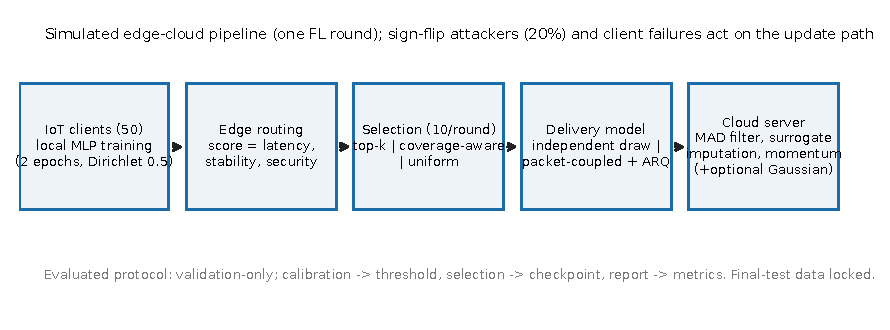
\includegraphics[width=\textwidth]{fig01_pipeline}
\caption{Simulated pipeline of one round and the evaluation protocol (schematic; every block is specified in Secs.~\ref{sec:network}--\ref{sec:data}).}\label{fig:pipeline}
\end{figure}
\section{Federated learning and aggregation methodology}
\label{sec:method}
\textbf{Learning.} Each client trains a 3-layer MLP (128--96--64, dropout 0.2) for 2 local epochs (Adam optimiser, learning rate $3\!\times\!10^{-4}$, batch 256) from the current global weights $w_t$ and returns $\Delta_i=w_i-w_t$. Data are partitioned across 50 clients with a Dirichlet allocation \cite{hsu2019measuring} ($\alpha=0.5$, at least 100 samples per client), 10 clients per round, 30 rounds.

\textbf{Genuine and surrogate updates.} A selected client contributes a \emph{genuine} update if it neither fails nor loses its update in transit. For each missing client, \emph{median-based surrogate imputation} inserts the coordinate-wise median of the available healthy updates (at least two are required) with weight $0.5\,n_i$. A surrogate is a statistical stand-in; it carries no information about the missing client's data, and "recovery of the client's contribution" is not claimed. All surrogates of a round are identical vectors. In the \RefA\ pipeline surrogates are added \emph{before} filtering; in \Cor\ the filter statistics use genuine updates only and surrogates are built from the retained genuine updates (post-filter), with their collective weight share capped at 0.10.

\textbf{Median/MAD filter.} With $c$ the coordinate-wise median of the vectors and $d_i=\lVert\Delta_i-c\rVert_2$, update $i$ is kept iff
\begin{equation}
d_i\le\operatorname{med}(d)+k\,(1.4826\,\operatorname{MAD}(d)+10^{-12}),\qquad k=2.5,
\end{equation}
with $\operatorname{MAD}(d)=\operatorname{med}|d_i-\operatorname{med}(d)|$ \cite{rousseeuw1993mad}; if nothing is kept, the update with the smallest $d_i$ is retained. The aggregate is the sample-weighted mean of kept updates, $\bar\Delta=\sum a_i\Delta_i$. A round with no delivered update leaves the model and the momentum buffer unchanged. This is the classical median/MAD rule; we claim no new estimator. \textbf{Server momentum.} $v\leftarrow\mu v+\bar\Delta$, $w_{t+1}=w_t+\eta_s v$ with $\mu=0.9$, $\eta_s=0.5$.

\textbf{Optional Gaussian perturbation.} The kept updates are clipped to $\ell_2$ norm $C=0.1$, the weights are projected onto a per-client cap of 0.1 (the smallest feasible cap $1/n$ is used when fewer than ten updates are kept), averaged, and Gaussian noise of standard deviation $z\,C\,\max_i a_i$ is added to the aggregate, with $z$ calibrated so that a diagnostic Renyi-DP accountant \cite{mironov2017renyi,zhu2019poisson} with sampling rate $q=0.2$, $T=30$, $\delta=10^{-5}$ reports $\hat\varepsilon\approx10$. \emph{This value is not a privacy guarantee}: selection is deterministic (no subsampling amplification), the filter and weights are data-dependent and unaccounted for, and the server sees unperturbed updates (run records state \texttt{subsampling\_amplification\_valid}$=$\texttt{false}).

\textbf{Implementation defect in the Gaussian path (Phase 8 finding).} In the historical Gaussian arms the collective surrogate cap of \Cor\ was undone by the per-client projection above: when fewer than ten updates survive (71\% of rounds in UNSW-NB15, 79\% in CICIoT2023) the projection is uniform, and the realised surrogate share of the aggregate was $0.476$/$0.480$ instead of $\le0.10$ ($0.096$/$0.097$ without Gaussian noise), although the run records \texttt{surrogate\_cap\_applied}$=$\texttt{True}. A default-off variant that enforces the group cap (\texttt{preserve\_surrogate\_cap}) exists in the code base but \emph{has not been run}; all Gaussian results below are historical, defective-path results and their gap to the noise-free arms is not purely a noise cost.

\textbf{Pipeline variants.} Table~\ref{tab:config} lists the configurations. \RefA\ = top-k selection, independent-draw delivery, pre-filter surrogates, no cap, sample-proportional weights, momentum 0.9. \Cor\ bundles coverage-aware selection, packet-coupled delivery, genuine-only filter with post-filter surrogates and the 0.10 surrogate cap. The ten \texttt{ctl\_*} arms change exactly one factor of \RefA. \Guard\ (a follow-up, Sec.~\ref{sec:guard}) abstains when fewer than three genuine updates arrive.

\begin{table}[t]\centering\scriptsize
\caption{Arm configurations (UNSW-NB15 configs; CICIoT2023 differs only in the dataset block). Source: \texttt{configs/phase6c/}, generated into \texttt{docs/phase8/tables/T6\_baseline\_configuration\_matrix\_phase6c.csv}. All attack arms use 20\% sign-flip (scale 5) and failure probability 0.1 unless noted.}\label{tab:config}
\resizebox{\textwidth}{!}{\begin{tabular}{@{}lllllllllc@{}}\toprule
Arm & Aggregation & Selection & Delivery & Impute & Surrogates & Sur.\ cap & Weights & Momentum & DP\\\midrule
corrected & distance\_filter & coverage\_aware & packet-coupled & yes & post-filter & 0.1 & samples & 0.9 & none \\
corrected\_gaussian & distance\_filter & coverage\_aware & packet-coupled & yes & post-filter & 0.1 & samples & 0.9 & central\_client \\
ctl\_delivery\_coupled & distance\_filter & top\_k & packet-coupled & yes & pre-filter & -- & samples & 0.9 & none \\
ctl\_imputation\_none & distance\_filter & top\_k & independent & no & pre-filter & -- & samples & 0.9 & none \\
ctl\_momentum0\_lr0p5 & distance\_filter & top\_k & independent & yes & pre-filter & -- & samples & 0.0 & none \\
ctl\_selection\_coverage & distance\_filter & coverage\_aware & independent & yes & pre-filter & -- & samples & 0.9 & none \\
ctl\_selection\_uniform & distance\_filter & uniform\_random & independent & yes & pre-filter & -- & samples & 0.9 & none \\
ctl\_weighting\_uniform & distance\_filter & top\_k & independent & yes & pre-filter & -- & uniform & 0.9 & none \\
reference & distance\_filter & top\_k & independent & yes & pre-filter & -- & samples & 0.9 & none \\
reference\_gaussian & distance\_filter & top\_k & independent & yes & pre-filter & -- & samples & 0.9 & central\_client \\
robust\_random\_no\_imputation & distance\_filter & uniform\_random & independent & no & pre-filter & -- & samples & 0.9 & none \\
scenario\_fedavg\_random & fedavg & uniform\_random & independent & no & pre-filter & -- & samples & 0.9 & none \\
scenario\_fedavg\_topk & fedavg & top\_k & independent & no & pre-filter & -- & samples & 0.9 & none \\
\bottomrule\end{tabular}
}
\end{table}

\section{Datasets, partitions and evaluation protocol}
\label{sec:data}
\textbf{UNSW-NB15} \cite{moustafa2015unsw}. The official training CSV (175{,}341 rows, SHA-256 \texttt{bec7dd5e\dots}) is split predictor-vector-group-disjointly into 150{,}293 training rows (48{,}000 benign, 102{,}293 attack) and a validation pool of 25{,}048 rows, which is split again into three group-disjoint partitions of $\approx$8{,}350 rows: \emph{calibration} (threshold), \emph{selection} (best checkpoint) and \emph{report} (all reported metrics; 2{,}666 benign). Raw 42 features expand to 194 after one-hot encoding of \texttt{proto}, \texttt{service}, \texttt{state}; preprocessing is fitted on the training rows only. The official testing CSV is not used.

\textbf{CICIoT2023} \cite{neto2023ciciot}. We use a capture-group-aware prepared version (926{,}133 training rows, 499{,}097 benign; 146{,}626 validation rows split into three partitions of $\approx$48{,}875 rows each with only $\approx$1{,}564 benign rows per partition; 39 features) whose content hashes are locked in the manifest. Provenance caveats: the files are byte-equivalent to a third-party release and their official provenance is unverified; labels were inferred from file/class names; there are no device identifiers, so the split is \emph{not} device-held-out; the benign prevalence differs strongly between training (53.9\%) and validation (3.2\%); AUC is near its ceiling ($\approx0.996$), so CICIoT2023 discriminates poorly between arms; and the CICIoT2023 and UNSW-NB15 network traces are identical, so the two datasets are not independent network evidence.

\textbf{Threshold and metrics.} For each evaluated model the decision threshold is chosen on the calibration partition as the point with the highest recall subject to FPR $\le0.15$ and recall $\ge0.6$ (ties: F1, balanced accuracy, closeness to 0.5; infeasible cases fall back to the FPR cap and are flagged). The threshold is then applied unchanged to the report partition. Consequently the report-partition FPR is $\approx0.14$--$0.15$ for essentially every arm and \emph{carries no information about differences between arms}; FPR transfer to unseen data is not tested here. \emph{Best} denotes the report-partition metrics of the checkpoint (round) that maximises AUC on the selection partition; \emph{last} denotes round 30. Both are always reported, because the best checkpoint hides last-round collapse. A \emph{collapse} is a last-round AUC below 0.80 (Phase 6C) or, in the pre-registered follow-up, last-round AUC $<0.90$ or a maximal mean training loss $>100$.

\textbf{Audited metrics.} After Phase 6C a defect was found in metric evaluation: scores were clipped to $[10^{-7},1-10^{-7}]$ before comparison with a threshold selected on raw scores, so a threshold of exactly 1.0 predicted no positive (spurious $F_1=0$) and clipping created artificial ties. Training is bitwise unaffected (verified on 13 completed runs); the saved checkpoints of all 240 Phase 6C runs were re-evaluated. Best-checkpoint AUC changes by at most $0.0037$ (F1 by $\le0.001$), but the last-round metrics of 12 runs change materially. Every number in this paper is the \emph{audited} value; the original values are kept in the ledger (\texttt{ledger\_per\_run\_phase6c.csv}). Whether the best-round \emph{selection} itself changed cannot be established, since per-round states were not stored (the best and runner-up rounds differ by $<0.001$ AUC in 182 of 240 runs).

\textbf{Statistics.} Five seeds (12--16; follow-up 17--21) are paired by seed. We report mean $\pm$ SD, per-seed values, paired mean differences with $t$-based 95\% intervals, wins and exact sign-flip $p$-values. With $n=5$ the smallest exact two-sided $p$ is $0.0625$; there is no multiplicity correction; every inferential statement is \emph{exploratory}. Seeds 12--21 have all been inspected; no seed is held out for confirmation.

\section{Results}
\label{sec:results}
\subsection{Detection performance and robustness to sign-flip attackers (RQ1)}
Table~\ref{tab:mainu} and Fig.~\ref{fig:best_last} give best-checkpoint and last-round performance. Without a defence, 20\% sign-flip clients destroy FedAvg: the UNSW-NB15 last-round AUC is $0.604\pm0.143$ (top-k) and $0.649\pm0.175$ (random), with 5/5 and 4/5 runs collapsing; on CICIoT2023 all ten undefended runs end at last-round AUC between $0.31$ and $0.76$ although their best checkpoints reach $0.945$--$0.996$ (best-checkpoint reporting hides the collapse). The MAD filter with server momentum restores performance to the level of clean FedAvg: UNSW-NB15 best AUC $0.9838$ (\RefA) vs.\ $0.9843$ (clean FedAvg; paired difference $-0.0005$, 95\% CI $[-0.0032,0.0022]$, 2/5 seeds in favour of \RefA), and $0.9962$ on CICIoT2023. Relative to undefended top-k FedAvg the best-checkpoint gain is $+0.097$ and the last-round gain $+0.378$ (5/5 seeds, $p=0.0625$, the minimum attainable). Centralised training gives $0.991$ (UNSW-NB15). Because every threshold is set to FPR $\approx0.15$, recall and F1 follow AUC.

\begin{table}[t]\centering\scriptsize
\caption{UNSW-NB15, Phase 6C, seeds 12--16, report partition, audited metrics, mean$\pm$SD. Collapsed = last-round AUC $<0.80$. Source: \texttt{Phase9\_Manuscript\_Revision/ledger/ledger\_arm\_summary\_phase6c.csv}.}\label{tab:mainu}
\resizebox{\textwidth}{!}{\begin{tabular}{@{}lcccccc@{}}\toprule
Arm & AUC best & AUC last & F1 best & Recall best & FPR best & Collapsed\\
\midrule
Centralized (no FL, clean) & 0.9911$\pm$0.0005 & 0.9912$\pm$0.0004 & 0.962 & 0.989 & 0.143 & 0/5 \\
FedAvg, clean & 0.9843$\pm$0.0029 & 0.9826$\pm$0.0051 & 0.954 & 0.973 & 0.142 & 0/5 \\
FedAvg, random selection, attack & 0.8752$\pm$0.0863 & 0.6493$\pm$0.1749 & 0.722 & 0.636 & 0.146 & 4/5 \\
FedAvg, top-k selection, attack & 0.8870$\pm$0.0856 & 0.6043$\pm$0.1430 & 0.770 & 0.699 & 0.142 & 5/5 \\
MAD filter, random selection, no imputation & 0.9825$\pm$0.0018 & 0.9770$\pm$0.0083 & 0.953 & 0.971 & 0.143 & 0/5 \\
Reference & 0.9838$\pm$0.0029 & 0.9826$\pm$0.0045 & 0.954 & 0.975 & 0.145 & 0/5 \\
Corrected & 0.9756$\pm$0.0067 & 0.9674$\pm$0.0251 & 0.948 & 0.964 & 0.147 & 0/5 \\
Reference + Gaussian & 0.9419$\pm$0.0166 & 0.9285$\pm$0.0187 & 0.900 & 0.878 & 0.149 & 0/5 \\
Corrected + Gaussian & 0.9406$\pm$0.0222 & 0.8890$\pm$0.1148 & 0.897 & 0.870 & 0.148 & 1/5 \\
Reference, 30\% failures & 0.9821$\pm$0.0029 & 0.9817$\pm$0.0035 & 0.952 & 0.967 & 0.139 & 0/5 \\
Corrected, 30\% failures & 0.9643$\pm$0.0153 & 0.8933$\pm$0.0862 & 0.928 & 0.926 & 0.145 & 1/5 \\
Reference, natural attackers & 0.9834$\pm$0.0042 & 0.9819$\pm$0.0059 & 0.954 & 0.975 & 0.146 & 0/5 \\
Corrected, natural attackers & 0.9690$\pm$0.0250 & 0.9368$\pm$0.0834 & 0.930 & 0.932 & 0.146 & 1/5 \\
\bottomrule\end{tabular}
}
\end{table}
\begin{table}[t]\centering\scriptsize
\caption{CICIoT2023 (capture-group split, AUC near ceiling, provenance unverified); otherwise as Table~\ref{tab:mainu}.}\label{tab:maincic}
\resizebox{\textwidth}{!}{\begin{tabular}{@{}lcccccc@{}}\toprule
Arm & AUC best & AUC last & F1 best & Recall best & FPR best & Collapsed\\
\midrule
Centralized (no FL, clean) & 0.9974$\pm$0.0002 & 0.9973$\pm$0.0002 & 0.995 & 0.994 & 0.144 & 0/5 \\
FedAvg, clean & 0.9962$\pm$0.0004 & 0.9960$\pm$0.0006 & 0.993 & 0.991 & 0.146 & 0/5 \\
FedAvg, random selection, attack & 0.9930$\pm$0.0015 & 0.5516$\pm$0.1154 & 0.990 & 0.986 & 0.140 & 5/5 \\
FedAvg, top-k selection, attack & 0.9813$\pm$0.0211 & 0.4625$\pm$0.0843 & 0.979 & 0.965 & 0.151 & 5/5 \\
MAD filter, random selection, no imputation & 0.9962$\pm$0.0003 & 0.9958$\pm$0.0007 & 0.993 & 0.992 & 0.147 & 0/5 \\
Reference & 0.9962$\pm$0.0003 & 0.9960$\pm$0.0006 & 0.993 & 0.992 & 0.144 & 0/5 \\
Corrected & 0.9960$\pm$0.0003 & 0.9949$\pm$0.0014 & 0.993 & 0.991 & 0.147 & 0/5 \\
Reference + Gaussian & 0.9930$\pm$0.0014 & 0.9931$\pm$0.0016 & 0.991 & 0.987 & 0.141 & 0/5 \\
Corrected + Gaussian & 0.9939$\pm$0.0010 & 0.9939$\pm$0.0010 & 0.991 & 0.987 & 0.142 & 0/5 \\
Reference, 30\% failures & 0.9960$\pm$0.0005 & 0.9959$\pm$0.0005 & 0.993 & 0.991 & 0.144 & 0/5 \\
Corrected, 30\% failures & 0.9957$\pm$0.0008 & 0.9767$\pm$0.0385 & 0.993 & 0.991 & 0.147 & 0/5 \\
Reference, natural attackers & 0.9961$\pm$0.0004 & 0.9960$\pm$0.0005 & 0.993 & 0.991 & 0.141 & 0/5 \\
Corrected, natural attackers & 0.9959$\pm$0.0006 & 0.9921$\pm$0.0073 & 0.993 & 0.991 & 0.143 & 0/5 \\
\bottomrule\end{tabular}
}
\end{table}
\begin{figure}[t]\centering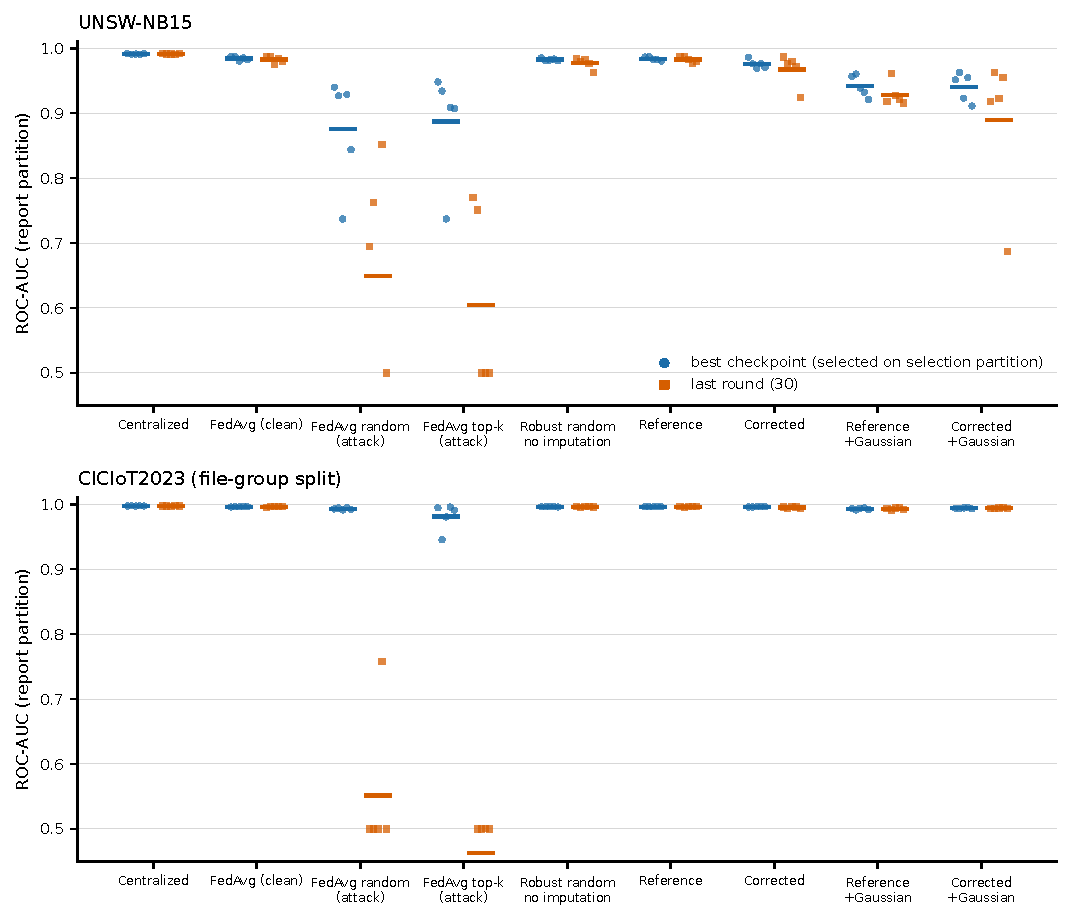
\includegraphics[width=\textwidth]{fig02_best_vs_last_auc}
\caption{Best-checkpoint (circles) and last-round (squares) ROC-AUC on the report partition for every main arm; dots are the five seeds, bars are means. Undefended FedAvg collapses at the last round. Source data: \texttt{figures/data/fig02\_best\_vs\_last\_auc.csv}.}\label{fig:best_last}
\end{figure}

\paragraph{Behaviour of the filter with few genuine updates.} Pooling all filter arms of Phase 6C, Table~\ref{tab:mad} shows that the filter has no discriminative power with one or two genuine updates (12/12 malicious updates accepted, 66 rounds), is unreliable with three (39.0\% of honest updates rejected, 30.6\% of malicious ones accepted) and still retains 14.1\% of the malicious updates when six or more genuine updates are present (Fig.~\ref{fig:mad}). A filter based on a median and a MAD needs several samples, so this is a design limitation of the rule rather than a bug; the pooled acceptance of all effective malicious updates is $15.0\%$ and the pooled rejection of honest updates $5.3\%$ (Phase 6C, 33{,}356 honest and 7{,}930 malicious update observations; the pooling mixes arms and is descriptive).
\begin{table}[t]\centering\scriptsize
\caption{MAD filter behaviour by number of genuine (non-surrogate) updates in a round, Phase 6C, all arms using the distance filter. Source: \texttt{docs/phase8/tables/T5b\_mad\_filter\_by\_number\_of\_real\_updates.csv}.}\label{tab:mad}
\begin{tabular}{@{}lccc@{}}\toprule
Genuine updates in round & Rounds & Honest rejected & Malicious accepted\\\midrule
1-2 & 66 & 4/102 (3.9\%) & 12/12 (100.0\%) \\
3 & 130 & 124/318 (39.0\%) & 22/72 (30.6\%) \\
4-5 & 1132 & 1105/4284 (25.8\%) & 180/908 (19.8\%) \\
>=6 & 4672 & 535/28652 (1.9\%) & 978/6938 (14.1\%) \\
\bottomrule\end{tabular}

\end{table}
\begin{figure}[t]\centering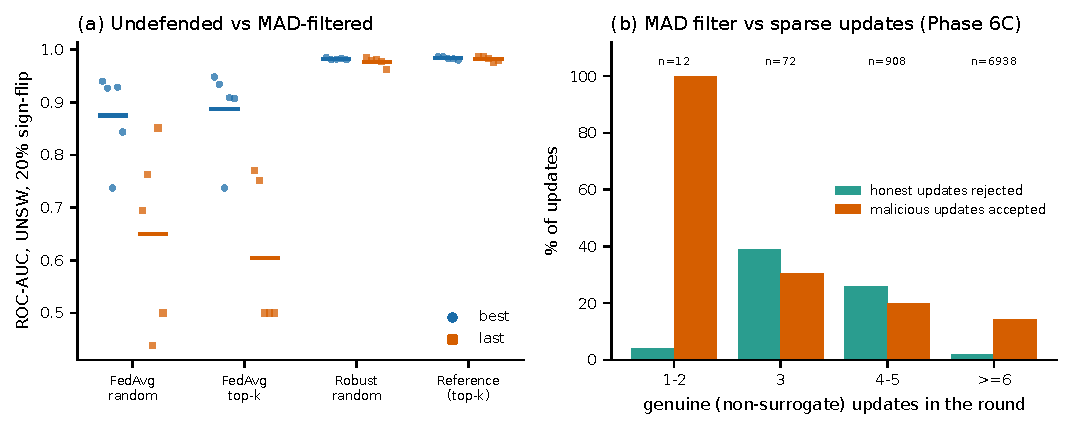
\includegraphics[width=\textwidth]{fig05_attack_robustness_and_mad}
\caption{(a) UNSW-NB15 ROC-AUC under 20\% sign-flip, undefended vs.\ filtered (circles best, squares last). (b) Honest-update rejection and malicious-update acceptance by the number of genuine updates in the round (numbers above bars: malicious update observations).}\label{fig:mad}
\end{figure}

\subsection{Routing: delivery reliability versus participation fairness (RQ2)}
\begin{table}[t]\centering\scriptsize
\caption{Network, delivery and participation by policy (means over 5 seeds). PDR = fraction of packets received at first transmission; Received/sel.\ = updates reaching the server per selected client (includes explicit failures); Gini over selection counts; Never sel.\ = clients (of 50) never selected in 30 rounds. Source: \texttt{ledger\_network\_fairness\_per\_run\_phase6c.csv}.}\label{tab:net}
\resizebox{\textwidth}{!}{\begin{tabular}{@{}llccccccc@{}}\toprule
Dataset & Policy & PDR & Delay (ms) & Path stab. & Transfer (Mbit/s) & Received/sel. & Gini & Never sel.\\\midrule
UNSW-NB15 & Uniform random & 0.782 & 81.5 & 0.855 & 14.9 & 0.706 & 0.205 & 0.0 \\
UNSW-NB15 & Coverage-aware & 0.833 & 76.3 & 0.904 & 17.1 & 0.743 & 0.486 & 8.0 \\
UNSW-NB15 & Top-k, independent draws (Reference) & 0.851 & 76.6 & 0.923 & 17.2 & 0.750 & 0.731 & 27.2 \\
UNSW-NB15 & Top-k, packet-coupled & 0.850 & 262.6 & 0.923 & 4.4 & 0.601 & 0.731 & 27.2 \\
UNSW-NB15 & Coverage-aware, packet-coupled (Corrected) & 0.834 & 267.6 & 0.904 & 3.9 & 0.557 & 0.486 & 8.0 \\
CICIoT2023 & Uniform random & 0.782 & 71.3 & 0.855 & 9.4 & 0.706 & 0.205 & 0.0 \\
CICIoT2023 & Coverage-aware & 0.833 & 65.8 & 0.904 & 10.8 & 0.743 & 0.486 & 8.0 \\
CICIoT2023 & Top-k, independent draws (Reference) & 0.851 & 65.9 & 0.923 & 10.9 & 0.750 & 0.731 & 27.2 \\
CICIoT2023 & Top-k, packet-coupled & 0.850 & 249.9 & 0.923 & 2.6 & 0.601 & 0.731 & 27.2 \\
CICIoT2023 & Coverage-aware, packet-coupled (Corrected) & 0.834 & 255.0 & 0.904 & 2.3 & 0.557 & 0.486 & 8.0 \\
\bottomrule\end{tabular}
}
\end{table}
Table~\ref{tab:net} and Fig.~\ref{fig:routing} show the trade-off. On the UNSW-NB15 trace, top-k selection improves mean PDR from $0.782$ to $0.851$ ($+8.8\%$ relative), end-to-end delay from $81.5$ to $76.6$ ms ($-6.0\%$), path stability from $0.855$ to $0.923$ and transfer efficiency from $14.9$ to $17.2$ Mbit/s ($+15.5\%$) relative to uniform selection (CICIoT2023, same trace: delay $-7.5\%$, transfer $+16.6\%$; payload size differs). These gains come with severe participation inequality: 27.2 of 50 clients are never selected (Gini $0.731$) versus none under uniform selection (Gini $0.205$). Coverage-aware selection sits in between (PDR $0.833$, delay $76.3$ ms, Gini $0.486$, 8.0 never selected). Detection quality is not measurably affected by the policy: best-AUC differences to \RefA\ are $-0.0023$ (uniform) and $-0.0009$ (coverage-aware) on UNSW-NB15 and $\le0.0001$ on CICIoT2023 (Table~\ref{tab:abl}); the mean recall of never-selected clients is $0.975$ versus $0.976$ for selected clients, so on these partitions the fairness cost is one of participation, not of accuracy (the scenario with correlated route quality and label distribution was not simulated). Because the attacker exposure is fixed by design, the exposure-controlled arms cannot show attacker avoidance; in the natural-attacker arms the malicious share of the selected clients is $0.195$ (top-k) vs.\ $0.188$ (uniform): the security input does not steer selection away from attackers.

Our earlier manuscript reported larger relative gains (e.g.\ delay $-26.6\%$, PDR $+13.4\%$, path stability $+62.8\%$ on CICIoT2023) against a baseline that we cannot reproduce with the present simulator; those figures are \emph{not retained}.

\begin{figure}[t]\centering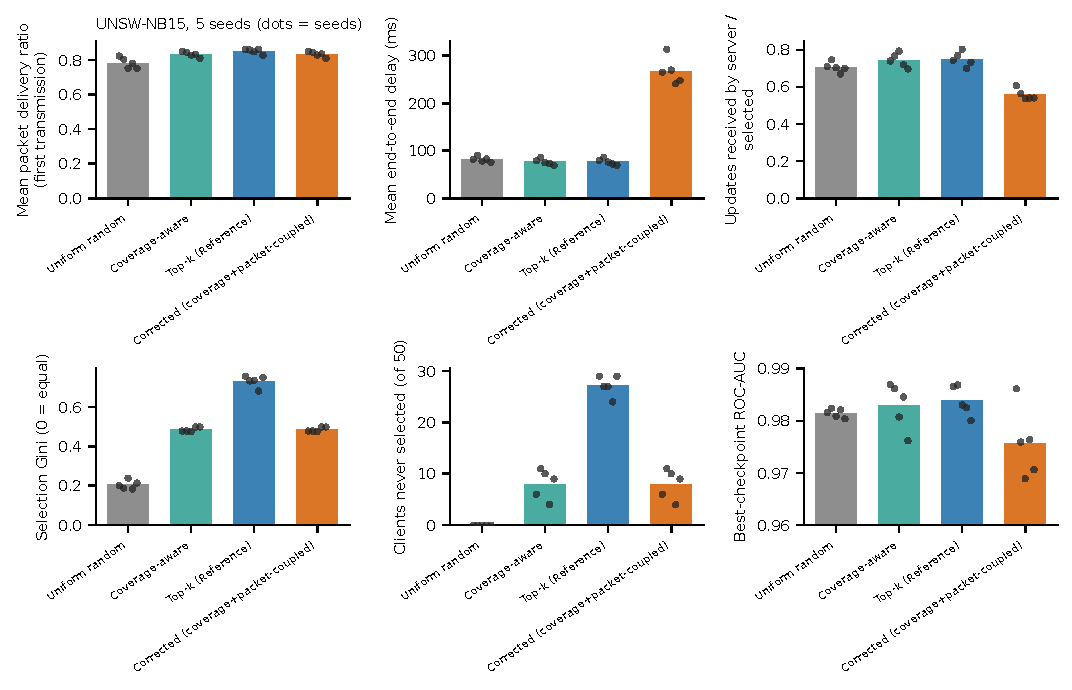
\includegraphics[width=\textwidth]{fig04_routing_fairness_tradeoff}
\caption{Selection policies on the UNSW-NB15 trace (dots: seeds). Top-k maximises PDR and minimises delay but starves clients; the AUC axis (last panel) is truncated to 0.96--0.99. Source: \texttt{figures/data/fig04\_routing\_fairness\_tradeoff.csv}.}\label{fig:routing}
\end{figure}

\subsection{Packet-coupled delivery, Corrected pipeline and controlled ablations}
\label{sec:ablation}
Packet-coupled delivery with at most two retransmissions changes the effective channel: for the same top-k selection the delivered fraction falls from $0.848$ to $0.681$, the delay rises from $76.6$ to $262.6$ ms and the transfer efficiency falls from $17.2$ to $4.4$ Mbit/s, while the first-transmission PDR is unchanged ($0.850$). \RefA\ (independent draws) and \Cor\ (packet-coupled) therefore do not face the same effective channel, and "reliability" claims for \Cor\ must be read against this: its delay is 3.5 times that of \RefA\ and its update delivery ratio is $0.626$ versus $0.848$ (Table~\ref{tab:net}; on-wire bytes of \Cor\ are $62.9$ MB against $52.4$ MB).

\Cor\ did not improve detection. Table~\ref{tab:paired}: UNSW-NB15 best-AUC difference $-0.0082$ (95\% CI $[-0.0147,-0.0017]$; worse in 5/5 seeds, exact $p=0.0625$), last-round $-0.0152$; CICIoT2023 $-0.0003$ (within noise). The single-factor ablations (Table~\ref{tab:abl}) all stay within about $0.005$ AUC of \RefA\ except momentum 0 with $\eta_s=5$ (last-round collapses of 2/5 CICIoT2023 runs); no single factor reproduces the \Cor\ deficit, and interactions were not tested, so we cannot attribute it. We find no evidence that surrogate imputation helps: removing it changes best AUC by $-0.0016$ (UNSW-NB15) and $-0.0001$ (CICIoT2023), in the noise. Mechanistic correlates (not isolated causes): \Cor\ keeps fewer genuine updates per round, $4.63$ vs.\ $5.93$, and the realised surrogate share is $0.096$ vs.\ $0.221$ for \RefA.

\begin{table}[t]\centering\scriptsize
\caption{Paired AUC differences (mean [95\% $t$-CI] (seeds in which the first arm is better)), audited values, 5 seeds; exact sign-flip $p\ge0.0625$ everywhere, so all statements are exploratory. Source: \texttt{ledger\_paired\_contrasts\_phase6c\_audited.csv}.}\label{tab:paired}
\resizebox{\textwidth}{!}{\begin{tabular}{@{}lcccc@{}}\toprule
 & \multicolumn{2}{c}{UNSW-NB15} & \multicolumn{2}{c}{CICIoT2023}\\\cmidrule(lr){2-3}\cmidrule(lr){4-5}
Contrast (AUC difference) & best & last & best & last\\\midrule
Corrected $-$ Reference & -0.0082 [-0.0147,-0.0017] (0/5) & -0.0152 [-0.0442,+0.0139] (0/5) & -0.0003 [-0.0007,+0.0001] (1/5) & -0.0011 [-0.0025,+0.0004] (1/5) \\
Corrected $-$ Reference, 30\% failures & -0.0179 [-0.0394,+0.0037] (0/5) & -0.0884 [-0.1983,+0.0215] (0/5) & -0.0003 [-0.0009,+0.0002] (2/5) & -0.0192 [-0.0665,+0.0283] (0/5) \\
Corrected $-$ Reference, natural attackers & -0.0144 [-0.0414,+0.0126] (1/5) & -0.0451 [-0.1461,+0.0558] (1/5) & -0.0003 [-0.0008,+0.0002] (1/5) & -0.0039 [-0.0126,+0.0049] (1/5) \\
Reference $-$ undefended FedAvg (top-k) & +0.0968 [-0.0084,+0.2020] (5/5) & +0.3782 [+0.2053,+0.5512] (5/5) & +0.0149 [-0.0111,+0.0410] (5/5) & +0.5334 [+0.4287,+0.6382] (5/5) \\
Reference $-$ clean FedAvg & -0.0005 [-0.0032,+0.0022] (2/5) & +0.0000 [-0.0069,+0.0070] (2/5) & +0.0001 [-0.0002,+0.0004] (3/5) & -0.0000 [-0.0010,+0.0010] (3/5) \\
Gaussian cost, Reference & -0.0419 [-0.0590,-0.0249] (0/5) & -0.0541 [-0.0749,-0.0333] (0/5) & -0.0032 [-0.0049,-0.0016] (0/5) & -0.0029 [-0.0042,-0.0016] (0/5) \\
Gaussian cost, Corrected & -0.0350 [-0.0579,-0.0121] (0/5) & -0.0784 [-0.1925,+0.0356] (0/5) & -0.0021 [-0.0031,-0.0011] (0/5) & -0.0010 [-0.0020,-0.0000] (0/5) \\
\bottomrule\end{tabular}
}
\end{table}
\begin{table}[t]\centering\scriptsize
\caption{Single-factor ablations: best/last AUC difference to \RefA\ (seeds better), UNSW-NB15 and CICIoT2023. Source: ledger paired contrasts; momentum-0/$\eta_s=5$ from the arm summary.}\label{tab:abl}
\resizebox{\textwidth}{!}{\begin{tabular}{@{}lcccc@{}}\toprule
 & \multicolumn{2}{c}{UNSW-NB15} & \multicolumn{2}{c}{CICIoT2023}\\\cmidrule(lr){2-3}\cmidrule(lr){4-5}
Single change to Reference & best & last & best & last\\\midrule
Uniform selection & -0.0023 (1/5) & -0.0091 (1/5) & -0.0001 (2/5) & -0.0001 (2/5) \\
Coverage-aware selection & -0.0009 (2/5) & -0.0024 (3/5) & -0.0001 (1/5) & +0.0001 (2/5) \\
Packet-coupled delivery (ARQ) & -0.0050 (1/5) & -0.0056 (2/5) & -0.0003 (0/5) & -0.0006 (0/5) \\
No surrogate imputation & -0.0016 (2/5) & -0.0004 (2/5) & -0.0001 (0/5) & -0.0000 (3/5) \\
Real-only filter, post-filter surrogates & -0.0017 (3/5) & -0.0001 (2/5) & -0.0001 (1/5) & -0.0000 (2/5) \\
Surrogate cap 0.10 & -0.0003 (1/5) & -0.0009 (1/5) & -0.0000 (2/5) & -0.0001 (1/5) \\
Uniform client weights & -0.0038 (1/5) & -0.0004 (1/5) & -0.0003 (1/5) & -0.0001 (1/5) \\
No server momentum ($\mu{=}0$, $\eta_s{=}0.5$) & -0.0010 (2/5) & +0.0001 (3/5) & -0.0000 (2/5) & +0.0002 (2/5) \\
No server momentum ($\mu{=}0$, $\eta_s{=}5$) & -0.0041 & -0.0402 & -0.0036 & -0.2653 \\
\bottomrule\end{tabular}
}
\end{table}
\begin{figure}[t]\centering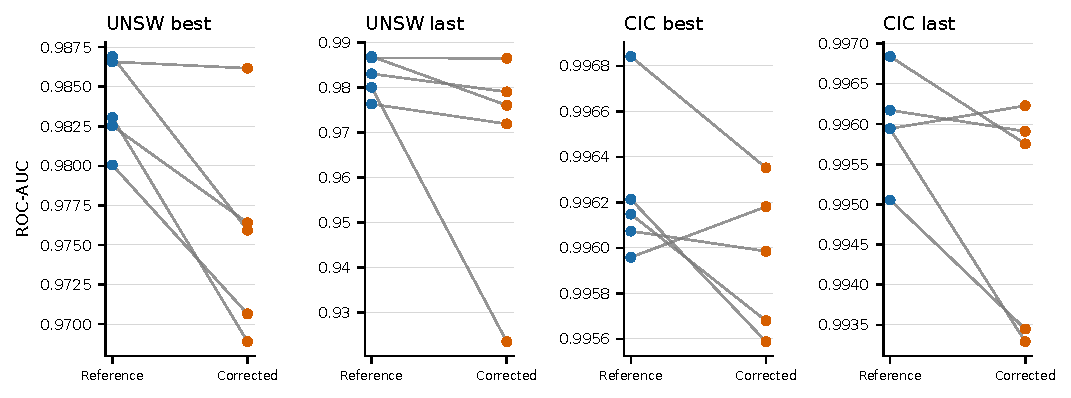
\includegraphics[width=0.85\textwidth]{fig03_reference_vs_corrected_paired}
\caption{Reference vs.\ Corrected paired by seed (ROC-AUC). Corrected is not better in any seed on UNSW-NB15 at the best checkpoint.}\label{fig:paired}
\end{figure}

\subsection{Failures and the minimum-real-update guard (RQ3)}
\label{sec:guard}
Under 30\% client failures, \RefA\ remains stable (UNSW-NB15 last AUC $0.9817\pm0.0035$ in Phase 6C) whereas \Cor\ degrades (last AUC $0.893\pm0.086$, 1/5 runs collapsed; paired last-round difference $-0.088$, 95\% CI $[-0.198,+0.022]$, 5/5 seeds worse); CICIoT2023 last-round $-0.019$. We hypothesised that the instability comes from rounds with very few genuine updates, and pre-registered a follow-up on new seeds 17--21 (UNSW-NB15, 8 arms $\times$ 5 seeds, manifest locked before the runs): \Guard\ makes the server abstain when 1 or 2 genuine updates arrive (value 3, chosen as the mathematical minimum of the median/MAD rule, not tuned). The primary contrast was \Guard\ versus \Cor\ under 30\% failures; support required no more collapses, mean last-round AUC gain $\ge+0.005$ in at least 4/5 seeds, and a best-checkpoint drop $\le0.002$.

Table~\ref{tab:p7b} and Fig.~\ref{fig:guard} give the outcome. Collapses fell from 2 to 1 and the mean last-round AUC rose from $0.840$ to $0.926$, but the guard was better in only 3/5 seeds (one equal, one worse by $0.147$, a new collapse), so the pre-registered criterion was \emph{not met}. The mean gain is carried by seed 17, whose outcome was seen before the follow-up was completed (and part of seed 18, observed during the diagnosis of the metric defect); excluding it the mean last-round change is $-0.007$. Without injected failures the guard is inert in 4 of 5 seeds (skipped rounds: 2 and 17 in the two guarded arms), and in the packet-coupled control it never activates. Run to completion with the repaired metrics, the same training as the earlier, defective-metric attempt gave identical models (verified for 13 runs). \RefA\ remains the more stable pipeline ($0.976\pm0.006$ last AUC at 30\% failures). We therefore do \emph{not} recommend the guard and make no claim that it improves the algorithm.
\begin{table}[t]\centering\scriptsize
\caption{Follow-up on new seeds 17--21 (UNSW-NB15, audited metric code). Collapse = last-round AUC $<0.90$ or maximal training loss $>100$. Source: \texttt{ledger\_per\_run\_phase7b.csv}.}\label{tab:p7b}
\resizebox{\textwidth}{!}{\begin{tabular}{@{}lccccccc@{}}\toprule
Arm (UNSW, seeds 17--21) & AUC best & AUC last & F1 best & F1 last & Recall best & Collapses & Skipped rounds\\\midrule
Reference & 0.9798$\pm$0.0074 & 0.9661$\pm$0.0255 & 0.948 & 0.936 & 0.964 & 0/5 & 0 \\
Corrected & 0.9694$\pm$0.0234 & 0.9496$\pm$0.0428 & 0.933 & 0.903 & 0.940 & 1/5 & 0 \\
Corrected + Guard & 0.9781$\pm$0.0052 & 0.9691$\pm$0.0116 & 0.948 & 0.930 & 0.966 & 0/5 & 2 \\
Reference, 30\% failures & 0.9757$\pm$0.0091 & 0.9760$\pm$0.0056 & 0.945 & 0.948 & 0.960 & 0/5 & 0 \\
Corrected, 30\% failures & 0.9013$\pm$0.1541 & 0.8401$\pm$0.2269 & 0.912 & 0.914 & 0.945 & 2/5 & 0 \\
Corrected + Guard, 30\% failures & 0.9631$\pm$0.0313 & 0.9261$\pm$0.0637 & 0.927 & 0.823 & 0.926 & 1/5 & 17 \\
Packet-coupled control & 0.9768$\pm$0.0076 & 0.9763$\pm$0.0053 & 0.950 & 0.948 & 0.969 & 0/5 & 0 \\
Packet-coupled + Guard & 0.9768$\pm$0.0076 & 0.9763$\pm$0.0053 & 0.950 & 0.948 & 0.969 & 0/5 & 0 \\
\bottomrule\end{tabular}
}
\end{table}
\begin{figure}[t]\centering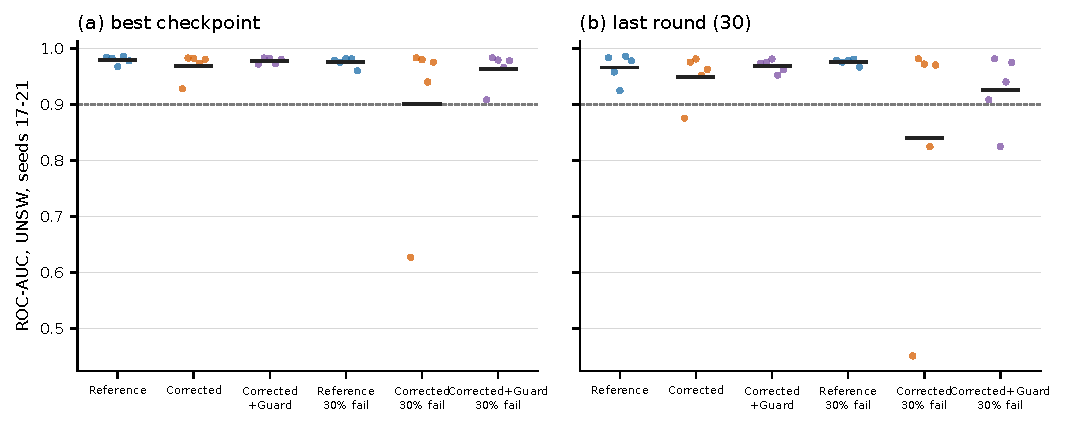
\includegraphics[width=\textwidth]{fig06_failures_and_guard_phase7b}
\caption{Per-seed AUC in the follow-up (dots: seeds 17--21; bars: means; dashed: 0.90). The guard removes the seed-17 collapse but creates one in seed 19.}\label{fig:guard}
\end{figure}

\subsection{Gaussian perturbation (historical, defective path)}
Noise costs accuracy: $-0.0419$ best AUC for \RefA\ (UNSW-NB15; 5/5 seeds; $0.9838\to0.9419$) and $-0.0032$ on CICIoT2023; $-0.0350$ and $-0.0021$ for \Cor. The reported accountant value $\hat\varepsilon\approx10$ is diagnostic only (Sec.~\ref{sec:method}). Because of the defect described there, the realised surrogate share is $0.476$ (UNSW-NB15) in \Cor{}+Gaussian (Fig.~\ref{fig:gauss}) and the gap is not a pure noise cost. The corrected variant was not evaluated.
\begin{figure}[t]\centering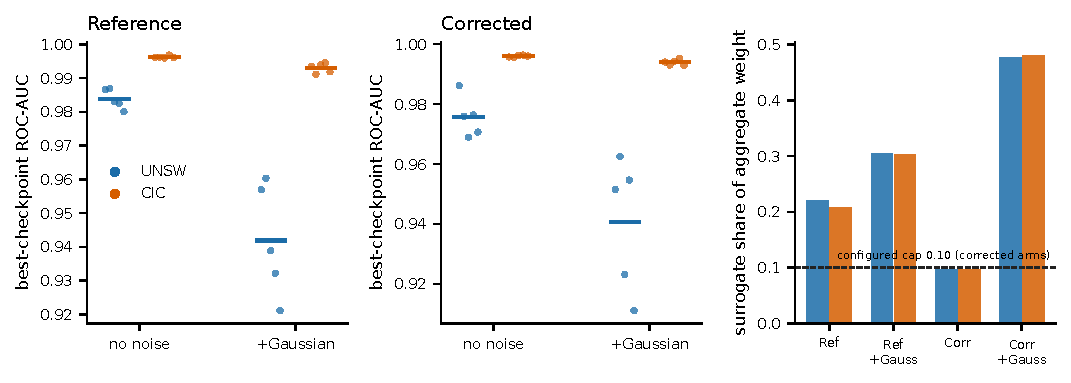
\includegraphics[width=\textwidth]{fig07_gaussian_and_surrogate_share}
\caption{Left/middle: best AUC without and with Gaussian perturbation. Right: realised surrogate share of the aggregate weight; the 0.10 cap is not enforced in the Gaussian path.}\label{fig:gauss}
\end{figure}

\section{Discussion and threats to validity}
\textbf{What is established.} Under a simulated 20\% sign-flip attacker, median/MAD filtering with server momentum is necessary and sufficient to keep federated IDS training at clean-FedAvg level on both datasets; network-aware top-k selection improves PDR and delay in the simulator but concentrates participation on a minority of clients; coverage-aware selection recovers part of the participation at no measurable detection cost. \textbf{What is not.} The revised pipeline (\Cor) is not better than \RefA\ in any measured dimension except participation fairness, and its extra delay is an artefact of a stricter delivery model; surrogate imputation shows no benefit; the guard failed; the Gaussian result is not privacy.

\textbf{Threats to validity.} (1) Five seeds: min $p=0.0625$, no multiplicity control; non-significance is not equivalence. (2) Validation-only evidence; the final test sets remain locked and untouched, so generalisation to the official test distributions is unknown, and operating-point FPR transfer is untested (the earlier manuscript's very high UNSW-NB15 test FPR for some proposed configurations is not re-examined). (3) One simulated network; the router uses true delivery probabilities; the security score carries no attacker information. (4) One attack family at one strength; no adaptive attacker, no sweep of the malicious fraction. (5) CICIoT2023: unverified provenance, no device holdout, severe prior shift, near-ceiling AUC; identical network trace to UNSW-NB15. (6) \Cor\ is a bundle, ablations are single-factor from \RefA\ only. (7) Seeds 12--21 have been inspected; the \Guard\ outcome of seed 17 and part of seed 18 was seen before completion. (8) Metric defect: after the audit, best-round selection may differ in some runs. (9) Hyper-parameters ($k$, $\lambda$, momentum, caps) were fixed and not studied; no resource measurement on edge hardware.

\section{Conclusion}
In a reproducible simulation, robust median/MAD aggregation with momentum protects federated IDS training against sign-flip clients, while network-aware client selection trades participation fairness for delivery reliability. A bundle of mechanisms intended to improve the pipeline did not, and a pre-registered guard did not meet its criterion. These measured limits, rather than a new estimator or a privacy claim, are the contribution; confirming them on held-out seeds, other attacks and the locked final-test data remains future work.

\section*{Reproducibility and data availability}
Code, locked manifests with SHA-256 hashes, resumable runners, audited metric tables, figure source data and 155 unit tests are in the project repository (Phase~8 and Phase~9 branches; git tags \texttt{phase6c-final-results} and \texttt{phase7b-final-results}); the file \texttt{REPRODUCIBILITY.md} in the revision folder lists the commands. UNSW-NB15 and CICIoT2023 are public and are not redistributed. A previous Zenodo deposit (DOI 10.5281/zenodo.21131047) predates this study, and an updated deposit must be made before submission. Final-test data were not accessed. \textbf{Declarations} (funding, competing interests, author contributions) are to be completed by the authors.

\FloatBarrier
\bibliographystyle{elsarticle-num}
\bibliography{../bibliography/verified_references}
\end{document}
